\section{Data Mining}

To identify the best classification algorithm different available operators were used in Rapidminer.
First runs per algorithm were executed using the cross-validation operator. After recall, precision and accuracy scores were available the second phase began. During this phase different approaches are used to maximize the prediction result and finetune the performance scores based on the best suited algorithm identified in phase 1. In a third phase a new test data set were applied based on data from 2017 to check of overfitted models. \newline

In the following sections the different algorithms and their results of phase 1 are described. 
Afterwards in section \ref{sec:Evaluation} results are evaluated.
Finally, a discussion of results is written down in section \ref{sec:DiscussionResults}. 


\subsection{K-Nearest Neighbors (KNN)}
\label{sec:KNN}
K-Nearest Neighbors classifies unseen cases based on the k nearest neighbors. 
%As input to train our model FIFA 2019 data set is used. 
First, the ``optimize parameters" operator was applied for values of k between 1 and 100 as well as a 10-fold cross validation. The result of this optimization showed that the ideal value for k = 62 which provides an accuracy of 87.83\%. The best performing class was \textit{goalkeeper} with a precision of 100\% and the worst performing class was midfielder with a precision of 81.45\%. \\
Applying our model to the FIFA17 test data set the following results could be measured:\\
\begin{table}[H]
\label{Tab:knn}
\centering
\begin{tabular}{@{}lll@{}}
\toprule
                   & Training data & Test data \\ \midrule
Accuracy           & 87.83\%       & 87.37\%   \\
Weighted recall    & 88.46\%       & 87.92\%   \\
Weighted precision & 90.08\%       & 88.86\%   \\ \bottomrule
\end{tabular}
\caption{Results from KNN algorithm on training and test data}
\end{table}
In phase two of the mining process using KNN we started to optimize the algorithm by optimizing the attributes.
To do this we used the ``Optimize Selection'' and the ``Optimize Selection (Evolutionary)'' operator which determined the weight for the attributes based on the Gini Index and the Information Gain.
The optimal attributes are presented in table 4.
\begin{table}[H]
\begin{tabular}{p{3.5cm}|p{7.5cm}l|l}
\hline 
Optimize Selection (9) & Crossing, Finishing, HeadingAccuracy, ShortPassing, Dribbling, LongPassing, Vision, Marking, SlidingTackle\\
\hline
Information Gain (24)& Crossing, Finishing, HeadingAccuracy, ShortPassing, Volleys, Dribbling, FKAccuracy, LongPassing, BallControl, Acceleration, SprintSpeed, Agility, Balance, Jumping, Stamina, Strength, LongShots, Interceptions, Positioning, Composure, Marking, StandingTackle, SlidingTackle, Vision \\
\hline 
Gini Index (21) & Crossing, Finishing, HeadingAccuracy, ShortPassing, LongPassing, BallControl, Acceleration, SprintSpeed, Agility, Balance, Jumping, Stamina, Strength, LongShots, Interceptions, Positioning, Composure, Marking, StandingTackle, SlidingTackle, Vision\\ \hline
\end{tabular}
\label{Tab:knn2}
\caption{Selection of attributes}
\end{table}	
By selecting the attributes, the accuracy increased to 88.28 \% (Optimize Selection), 88.15 \% (Information Gain), 87.97\% (Gini Index). Table 5 shows the results on FIFA 2017 data set after the optimize selection.

\begin{table}[H]
\begin{tabular}{@{}llll@{}}
\toprule
                                        & Accuracy & Weighted Recall & Weighted Precision \\ \midrule
\multicolumn{1}{l|}{Optimize Selection} & 87.24\%  & 87.84\%         & 88.56\%            \\
\multicolumn{1}{l|}{Information Gain}          & 87.39\%  & 87.94\%         & 88.95\%            \\
\multicolumn{1}{l|}{Gini Index}         & 87.18\%  & 87.70\%         & 88.65\%            \\ \bottomrule
\end{tabular}
\label{Tab:KNNResults}
\caption{Results of KNN on test data}
\end{table}

As last optimization the ``Optimize Parameters" operator was used again, but only for the selected attributes with k values (1-100, 100 steps). This resulted to a k = 57 with the subset of attributes from the operator, and a k = 1 for both Information Gain and Gini Index. With this last optimization the test results couldn't be improved anymore and the accuracy dropped by 0.2\%.

\subsection{Decision Tree}

\subsection{Result using Gradient Boosted Trees}

The gradient boosted trees algorithm is used to create an ensemble of decision trees trough gradually improved estimations. The output is a classification model which can be applied to the test dataset for a prediction of the label attribute position\_grouped. 
One advantage is the written report about the weights of attributes with respect to the label attribute.~\cite{ref_rapidminergbt}
The number of trees was set to 30. The maximal depth was initially set to 15, while the best result were scored with a maximal depth of 30.
The number of bins was set to 30.  
The process was executed with different settings regarding the maximal depth of trees. In summary, allowing a higher maximal depth resulted in better scores for $R^2$, recall and precision. Result of this values are shown in table \ref{Tab:GBT}.


\begin{table}[]
\begin{tabular}{@{}lllllll@{}}
\textbf{Run} & \textbf{\begin{tabular}[c]{@{}l@{}}Max. \\ tree depth\end{tabular}} & \textbf{\begin{tabular}[c]{@{}l@{}}Number \\ of folds\end{tabular}} & \textbf{Recall} & \textbf{Precision} & \textbf{$R^2$} & \textbf{\begin{tabular}[c]{@{}l@{}}Mean squarred\\ error\end{tabular}} \\
1            & 10                                                                  & 15                                                                   & 88,21 \%               & 89,01 \%                  & 64,4 \%                       & 0.33733332                                                             \\
2            & 15                                                                  & 15                                                                  & 88,05 \%               & 88,68 \%                  & 65,3 \%                       & 0.3289592                                                              \\
3            & 25                                                                  & 15                                                                  & 88,09 \%               & 88,70 \%                  & 65,4 \%                       & 0.3286427                                                              \\
4            & 30                                                                  & 15                                                                  & 88.09\%               & 88.73 \%                  & 65,4 \% & 0.328648                                                                     
\end{tabular}
\label{Tab:GBT}
\caption{Performance results of gradient boosted trees}
\end{table}

As important attributes the following were highlighted in table \ref{Tab:GBTImportantAttributes}:

\begin{table}[]
\begin{tabular}{@{}llll@{}}
\toprule
Variable        & \begin{tabular}[c]{@{}l@{}}Relative \\ Importance\end{tabular} & \begin{tabular}[c]{@{}l@{}}Scales \\ Importance\end{tabular}    & Percentage \\ \midrule
SlidingTackle   & 43887.371094        & 1.000000 & 0.179607   \\
Skill Moves     & 40664.996094        & 0.926576                      & 0.166419   \\
LongPassing     & 27751.718750        & 0.632340                      & 0.113572   \\
LCB             & 23368.140625        & 0.532457                      & 0.095633   \\
HeadingAccuracy & 22303.111328        & 0.508190                      & 0.091274   \\
LAM             & 16302.590820        & 0.371464                      & 0.066717   \\
Finishing       & 9715.319336         & 0.221369                      & 0.039759   \\
Crossing        & 9004.551758         & 0.205174                      & 0.036851   \\
SprintSpeed     & 5180.378906         & 0.118038                      & 0.021200   \\
ShortPassing    & 3899.299316         & 0.088848                      & 0.015958   \\ \bottomrule
\end{tabular}
\label{Tab:GBTImportantAttributes}
\caption{Important Attributes according to gradient boosted trees algorithm}
\end{table}
\subsection{Deep Learning}

Test Paul.\\

\subsection{Support Vector Machines}
Support Vector Machines (SVM) is a linear model for classification and regression problems. The SVM Linear takes a set of input data and predicts, for each given input, which of the two possible classes comprises the input, making the SVM a non-probabilistic binary linear classifier \cite{ref_rapidminersvm}.
We use cross validation for estimating statistical performance, classification by regression to build a polynomial classification model through regression learner and SVM linear to build a model that assigns new examples into one category or the other.\\
 A change in the value of the parameter C of SVM, which is the complexity constant, sets the tolerance for misclassification in its parameters where higher C values allow for `softer' boundaries and lower values create `harder' boundaries \cite{ref_rapidminersvm}.  A complexity constant that is large will lead to overfitting and values that are too small may result in over-generalization.\\
The algorithm looks at the extreme cases and draws a decision boundary known as hyperplane. The result from the optimization provides C for SVM Linear with the best value of 1.0. 
Training SVM on the FIFA 2019 data set, as shown in the table 7, leads to an the overall accuracy of 85.06\%. The best performing class is goalkeeper with 99.95\% accuracy and the worst performing class is strikers with 79.65\% accuracy. Precision and recall of the training set are 86.44\% and 87.87\% respectively. 
Applying the model to the test data set provides an overall accuracy of 83,74\% as shown in table 7. The best performing class is Goalkeeper with 100\% accuracy and the worst performing class is Striker with 76.10\% accuracy. The precision and recall of the test set obtained are 85.42\% and 85.76\% respectively. 

\begin{table}[]
\centering
\begin{tabular}{@{}l|ll@{}}
\hline
                    & Training & Testing \\ \hline
Accuracy            & 85,06 \% & \textbf{83,74\%} \\ \hline
Accuracy Goalkeeper & 99,95\%  & 100\%   \\
Accuracy Defender   & 87,1\%   & 87,9\%  \\
Accuracy Strikers   & 83,57\%  & 76,1\%  \\
Accuracy Midfielder & 79,65\%  & 79,04\% \\ \hline
Weighted Precision  & 86,44\%  & 85,42\% \\
Weighted Recall     & 87,87\%  & 85,76\% \\ \hline
\end{tabular}
\label{Tab:SVM}
\caption{Comparison of results of support vector machine algorithm}
\end{table}

\subsection{Random Forest}

At the end, we applied the random forest classifier as our sixth classification algorithm. In
general, Random Forests are used in classification and regression problems~\cite{ref_rapidminerRandomForest}.
A random forest is an ensemble method which consists of a collection of
multiple random decision trees. In many data sets, the Random Forest perform better than
decision tree classifiers ~\cite{ref_Tan}. Each tree is generated by random vectors of the training data sets. The nodes in the decision
trees are represented by the attributes. \newline 
When applying the model to new examples, each tree predicts a class by following the branches of the decision tree. The output is a voting
classification model which combines the decision trees in the random forest which means that
each tree in this forest make a decision and the class with the most votes determines the final
class. The classification of the random forest varies less than of each random tree on its own,
because every classification in the random forest is treated equally important. ~\cite{ref_rapidminerRandomForest} \newline
To find the optimal
values Optimize Parameter operator ran with different
values for number of trees (20 to 90 in steps of 7 with linear scale) and maximal depth (0 to
100 in steps of 10 with linear scale). Using the accuracy as splitting criterion. The resulting
optimal values for number of trees is 90 and for maximal depth is 50 (as well as: 76 for
number of trees and 100 for maximal depth and 90 for number of trees and 50 for maximal
depth). For the first combination of values, an accuracy of 88.39\% was scored, weighted precision of
90.22\% and a weighted recall of 89.15\%. Our best performing class was again the goalkeeper with a
precision of 100\% and our worst performing class was again the midfielder with a precision
of 83.53\%. The model was tested with FIFA17 data for the three
value combinations mentioned above. Different splitting criterions beside
Accuracy like Gain ratio, Information gain and Gini index were tried. The best result was archieved with
76 trees and a maximal depth of 100, using Information Gain as splitting criterion. The
results for this value combination are shown in table \ref{tab:RandomForest}.

\begin{table}[]
\begin{tabular}{@{}llll@{}}
\toprule
Splitting criterion                            & Accuracy         & Weighted Recall  & Weighted Precision \\ \midrule
\multicolumn{1}{l|}{Accuracy}                  & 84,63\%          & 85,77\%          & 87,13\%            \\
\multicolumn{1}{l|}{Gain Ratio}                & 87,55\%          & 87,67\%          & 89,24\%            \\
\multicolumn{1}{l|}{\textbf{Information Gain}} & \textbf{88,67\%} & \textbf{89,25\%} & \textbf{89,81\%}   \\
\multicolumn{1}{l|}{GINI index}                & 88,62\%          & 89,23\%          & 89,70\%            \\ \bottomrule
\end{tabular}
\label{tab:RandomForest}
\caption{Results of random forest model on test data}
\end{table}



\subsection{Evaluation setup and results}
\label{sec:Evaluation}
\subsection{Discussion of results}
\label{sec:DiscussionResults}
The perfect classification of goalkeepers can be justified by strength and weaknesses of these football positions.

 Goalkeepers have low values regarding sliding tackle, skill moves, sprint speed, etc. A visualization in a coordination systems \ref{fig:VisualAttributes} shows that goalkeepers (black) have the biggest deficits in these and other attributes (values in the bottom left corner). Defenders (blue) are better in these categories than goalkeepers. While midfielder (green) and strikers (orange) have nearly same strengths (one dot on top of each other in middle and top right corner). 

\begin{figure}
\centering
  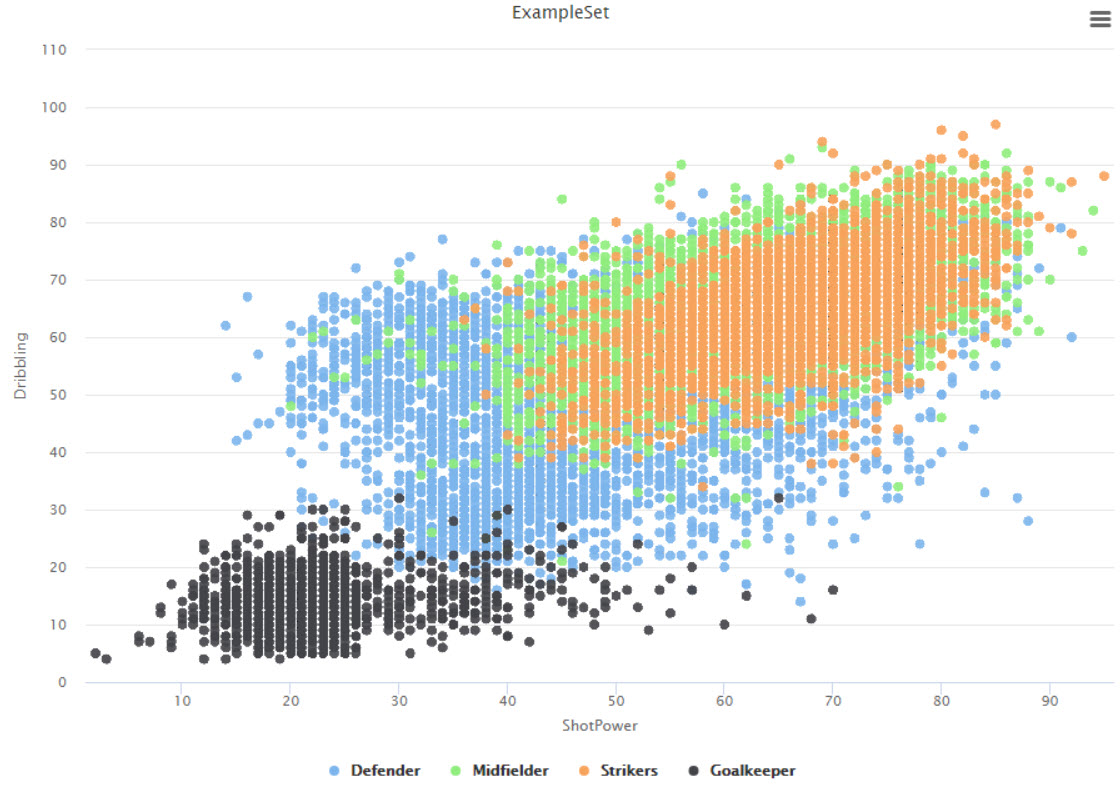
\includegraphics[width=8cm]{VisualizationAttributes.jpg}
  \caption{Visualization of two characteristics: dribbling and shot power}
  \label{fig:VisualAttributes}
\end{figure}

The result matches the expectations as the boundaries between strikers and midfielders are blurry. These two attributes are only an excerpt from more than 80 attributes but are typical for the data set.

As a conclusion, the data model to predict a soccer players position scores good result on the training and test data sets. Due to nearly identical attribute values for midfielders and strikers the accuracy decreased.